%%%%%%%%%%%%%%%%%%%%%%%% INICIO QUADRO 01 %%%%%%%%%%%%%%%%%%%%%%%%%%%%%%%
\begin{table}[ht]
  \centering
  \caption{Quadro 01}
  \label{Quadro_01}
  \begin{tabular}[t]{|ll|l|l|}
    \hline

    %%% PRÓXIMA LINHA
    \letraquadrada{A}   &   \em    &    \letraquadrada{B}    &    \letraquadrada{C}


    %%% PRÓXIMA LINHA
    \\
    \quadtitulo
    &
    \quadtitulo
    &
    \quadtitulo{Compasso}
    &
    \quadtitulo{Fórmula de compasso}


    %%% PRÓXIMA LINHA
    \\
    \begin[fragment]{lilypond}
      \transpose c c {
        \keepWithTag #'cl
        \include "notas-01.ly"
      }
    \end{lilypond}
    &
    \begin[fragment]{lilypond}
      \transpose c c { 
        \keepWithTag #'cl
        \include "notas-02.ly" 
      }
    \end{lilypond}
    &
    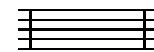
\includegraphics[scale=1]{compasso-vazio}
    &
    \includegraphics[scale=1]{4tempos-por-compasso}


    %%% PRÓXIMA LINHA
    \\
    \includegraphics[scale=3.15]{%#fig-posicoes#%-01}
    &
    \includegraphics[scale=3.15]{%#fig-posicoes#%-02}
    &
    \em
    &
    \em


    %%% PRÓXIMA LINHA
    \\
    \hline
    \letraquadrada{D}
    &
    \em
    &
    \letraquadrada{E}
    &
    \letraquadrada{F}


    %%% PRÓXIMA LINHA
    \\
    \quadtitulo{Semibreve}
    &
    \em
    &
    \quadtitulo{Mínima}
    &
    \quadtitulo{Pausa de semibreve}


    %%% PRÓXIMA LINHA
    \\
    \includegraphics[scale=1]{semibreve}
    &
    \em
    &
    \includegraphics[scale=1]{minima}
    &
    \includegraphics[scale=1]{semibreve-pausa}



    %%% FINAL DAS LINHAS
  \\
  \hline
  \end{tabular}
\end{table}    


%%%%%%%%%%%%%%%%%%%%%%%% FINAL QUADRO %%%%%%%%%%%%%%%%%%%%%%%%%%%%%%%%%%%

%%%%%%%%%%%%%%%%%%%%%%%% INICIO QUADRO 02 %%%%%%%%%%%%%%%%%%%%%%%%%%%%%%%

\begin{table}[ht]
  \centering
  \caption{Quadro 02}
  \label{Quadro_02}
  \begin{tabular}[t]{|l|l|l|}
    \hline

    %%% PRÓXIMA LINHA
    \letraquadrada{A}    &    \letraquadrada{B}    &    \letraquadrada{C}


    %%% PRÓXIMA LINHA
    \\
    \quadtitulo{Pausa de mínima}
    &
    \quadtitulo{Barra final}
    &
    \quadtitulo{Barra de compasso}


    %%% PRÓXIMA LINHA
    \\
    \includegraphics[scale=1]{minima-pausa}
    &
    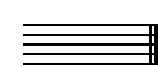
\includegraphics[scale=1]{barra-final}
    &
    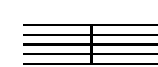
\includegraphics[scale=1]{barra-compasso}


    %%% PRÓXIMA LINHA
    \\
    \hline
    \letraquadrada{D}
    &
    \multicolumn{2}{|l|}{
    \letraquadrada{E}}
   

    %%% PRÓXIMA LINHA
    \\
    \quadtitulo{Semínima}
    &
    \multicolumn{2}{|l|}{
    \quadtitulo{Fórmula de compasso}}



    %%% PRÓXIMA LINHA
    \\
    \includegraphics[scale=1]{seminima}
    &
    \multicolumn{2}{|l|}{
    \includegraphics[scale=1]{formula-4tempos-por-compasso}}


    %%% FINAL DAS LINHAS
  \\
  \hline
  \end{tabular}
\end{table}    



%%%%%%%%%%%%%%%%%%%%%%%% FINAL QUADRO %%%%%%%%%%%%%%%%%%%%%%%%%%%%%%%%%%%

%%%%%%%%%%%%%%%%%%%%%%%% INICIO QUADRO 03 %%%%%%%%%%%%%%%%%%%%%%%%%%%%%%%

\begin{table}[ht]
  \centering
  \caption{Quadro 03}
  \label{Quadro_03}
  \begin{tabular}[t]{|l|l|l|}
    \hline

    %%% PRÓXIMA LINHA
    \letraquadrada{A}    &    \letraquadrada{B}    &    \letraquadrada{C}


    %%% PRÓXIMA LINHA
    \\
    \quadtitulo
    &
    \quadtitulo{Sinal de respiração}
    &
    \quadtitulo{Pauta ou pentagrama}


    %%% PRÓXIMA LINHA
    \\
    \begin[fragment]{lilypond}
      \transpose c c { 
        \keepWithTag #'cl
        \include "notas-03.ly" 
      }
    \end{lilypond}
    &
    \includegraphics[scale=1]{respiracao}
    &
    \includegraphics[scale=1]{pauta}

    %%% PRÓXIMA LINHA
    \\
    \includegraphics[scale=3.15]{%#fig-posicoes#%-03}
    &
    \em
    &
    \em


    %%% FINAL DAS LINHAS
  \\
  \hline
  \end{tabular}
\end{table}    


%%%%%%%%%%%%%%%%%%%%%%%% FINAL QUADRO %%%%%%%%%%%%%%%%%%%%%%%%%%%%%%%%%%%


%%%%%%%%%%%%%%%%%%%%%%%% INICIO QUADRO 04 %%%%%%%%%%%%%%%%%%%%%%%%%%%%%%%

\begin{table}[ht]
  \centering
  \caption{Quadro 04}
  \label{Quadro_04}
  \begin{tabular}[t]{|l|l|l|}
    \hline

    %%% PRÓXIMA LINHA
    \letraquadrada{A}    &    \letraquadrada{B}    &    \letraquadrada{C}


    %%% PRÓXIMA LINHA
    \\
    \quadtitulo
    &
    \quadtitulo{Pausa de semínima}
    &
    \quadtitulo{Fórmula de compasso}


    %%% PRÓXIMA LINHA
    \\
    \begin[fragment]{lilypond}
      \transpose c c { \keepWithTag #'cl
        \include "notas-04.ly" }
    \end{lilypond}
    &
    \includegraphics[scale=1]{seminima-pausa}
    &
    \includegraphics[scale=1]{formula-3tempos-por-compasso}


    %%% PRÓXIMA LINHA
    \\
    \includegraphics[scale=3.15]{%#fig-posicoes#%-04}
    &
    \em
    &
    \em

    %%% FINAL DAS LINHAS
    \\
    \hline
  \end{tabular}

  \begin{tabular}[t]{|l|l|}
    %%% PRÓXIMA LINHA

    \letraquadrada{D}
    &
    \letraquadrada{E}
   

    %%% PRÓXIMA LINHA
    \\
    \quadtitulo{Clave de sol}
    &
    \quadtitulo{Clave de fá}


    %%% PRÓXIMA LINHA
    \\
    \includegraphics[scale=1]{clave-sol}
    &
    \includegraphics[scale=1]{clave-fa}

    %%% FINAL DAS LINHAS
  \\
  \hline
  \end{tabular}
\end{table}    

%%%%%%%%%%%%%%%%%%%%%%%% FINAL QUADRO %%%%%%%%%%%%%%%%%%%%%%%%%%%%%%%%%%%



%%%%%%%%%%%%%%%%%%%%%%%% INICIO QUADRO 05 %%%%%%%%%%%%%%%%%%%%%%%%%%%%%%%

\begin{table}[ht]
  \centering
  \caption{Quadro 05}
  \label{Quadro_05}
  \begin{tabular}[t]{|l|l|l|}
    \hline

    %%% PRÓXIMA LINHA
    \letraquadrada{A}    &    \letraquadrada{B}    &    \letraquadrada{C}


    %%% PRÓXIMA LINHA
    \\
    \quadtitulo
    &
    \quadtitulo{Ligadura}
    &
    \quadtitulo{Fórmula de compasso}


    %%% PRÓXIMA LINHA
    \\
    \begin[fragment]{lilypond}
      \transpose c c {
        \keepWithTag #'cl
        \include "notas-05.ly"
      }
    \end{lilypond}
    &
    \includegraphics[scale=1]{ligadura-minima}
    &
    \includegraphics[scale=1]{formula-2tempos-por-compasso}


    %%% PRÓXIMA LINHA
    \\
    \includegraphics[scale=3.15]{%#fig-posicoes#%-05}
    &
    \em
    &
    \em
    %%% FINAL DAS LINHAS
    \\
    \hline
  \end{tabular}

  \begin{tabular}[t]{|l|l|}
    %%% PRÓXIMA LINHA

    \letraquadrada{D}
    &
    \letraquadrada{E}
   

    %%% PRÓXIMA LINHA
    \\
    \quadtitulo{Andamento}
    &
    \quadtitulo{Anacruse}


    %%% PRÓXIMA LINHA
    \\
    \includegraphics[scale=1]{andamento}
    &
    \includegraphics[scale=1]{anacruse5}

    %%% FINAL DAS LINHAS
  \\
  \hline
  \end{tabular}
\end{table}    

%%%%%%%%%%%%%%%%%%%%%%%% FINAL QUADRO %%%%%%%%%%%%%%%%%%%%%%%%%%%%%%%%%%%


%%%%%%%%%%%%%%%%%%%%%%%% INICIO QUADRO 06 %%%%%%%%%%%%%%%%%%%%%%%%%%%%%%%

\begin{table}[ht]
  \centering
  \caption{Quadro 06}
  \label{Quadro_06}
  \begin{tabular}[t]{|l|l|}
    \hline

    %%% PRÓXIMA LINHA
    \letraquadrada{A}    &    \letraquadrada{B}


    %%% PRÓXIMA LINHA
    \\
    \quadtitulo
    &
    \quadtitulo{Sinal de repetição}


    %%% PRÓXIMA LINHA
    \\
    \begin[fragment]{lilypond}
      \transpose c c {
        \keepWithTag #'cl
        \include "notas-06.ly"
      }
    \end{lilypond}
    &
    \includegraphics[scale=1]{sinal-repeticao}


    %%% PRÓXIMA LINHA
    \\
    \includegraphics[scale=3.15]{%#fig-posicoes#%-06}
    &
    \em

    %%% PRÓXIMA LINHA
    \\
    \hline
    \multicolumn{2}{|l|}{\letraquadrada{C}}

    %%% PRÓXIMA LINHA
    \\
    \multicolumn{2}{|l|}{\quadtitulo{Anacruse}}


    %%% PRÓXIMA LINHA
    \\
    \multicolumn{2}{|c|}{\includegraphics[scale=1]{anacruse6}}


    %%% FINAL DAS LINHAS
    \\
    \hline
  \end{tabular}
\end{table}    


%%%%%%%%%%%%%%%%%%%%%%%% FINAL QUADRO %%%%%%%%%%%%%%%%%%%%%%%%%%%%%%%%%%%


%%%%%%%%%%%%%%%%%%%%%%%% INICIO QUADRO 07 %%%%%%%%%%%%%%%%%%%%%%%%%%%%%%%

\begin{table}[ht]
  \centering
  \caption{Quadro 07}
  \label{Quadro_07}
  \begin{tabular}[t]{|l|l|l|}
    \hline

    %%% PRÓXIMA LINHA
    \letraquadrada{A}    &    \letraquadrada{B}    &    \letraquadrada{C}


    %%% PRÓXIMA LINHA
    \\
    \quadtitulo
    &
    \quadtitulo{Sinal de repetição}
    &
    \quadtitulo{Moderato}


    %%% PRÓXIMA LINHA
    \\
    \begin[fragment]{lilypond}
      \transpose c c {
        \keepWithTag #'cl
        \include "notas-07.ly"
      }
    \end{lilypond}
    &
    \includegraphics[scale=1]{sinal-repeticao7-1}
    &
    \includegraphics[scale=1]{moderato}


    %%% PRÓXIMA LINHA
    \\
    \includegraphics[scale=3.15]{%#fig-posicoes#%-07}
    &
    \includegraphics[scale=1]{sinal-repeticao7-2}
    &
    \em

    %%% FINAL DAS LINHAS
    \\
    \hline
  \end{tabular}
\end{table}    

%%%%%%%%%%%%%%%%%%%%%%%% FINAL QUADRO %%%%%%%%%%%%%%%%%%%%%%%%%%%%%%%%%%%

%%%%%%%%%%%%%%%%%%%%%%%% INICIO QUADRO 08 %%%%%%%%%%%%%%%%%%%%%%%%%%%%%%%

\begin{table}[ht]
  \centering
  \caption{Quadro 08}
  \label{Quadro_08}
  \begin{tabular}[t]{|l|l|l|}
    \hline

    %%% PRÓXIMA LINHA
    \letraquadrada{A}    &    \letraquadrada{B}    &    \letraquadrada{C}


    %%% PRÓXIMA LINHA
    \\
    \quadtitulo
    &
    \quadtitulo{Ponto de aumento}
    &
    \quadtitulo{Ligadura de prolongação}


    %%% PRÓXIMA LINHA
    \\
    \begin[fragment]{lilypond}
      \transpose c c {
        \keepWithTag #'cl
        \include "notas-08.ly"
      }
    \end{lilypond}
    &
    \includegraphics[scale=1]{minima-pontuada}
    &
    \includegraphics[scale=1]{minima-ligada-seminima}



    %%% PRÓXIMA LINHA
    \\
    \includegraphics[scale=3.15]{%#fig-posicoes#%-08}
    &
    \em
    &
    \em
    %%% FINAL DAS LINHAS
    \\
    \hline
  \end{tabular}

  \begin{tabular}[t]{|l|p{7cm}|}
    %%% PRÓXIMA LINHA

    \letraquadrada{D}
    &
    \letraquadrada{E}
   

    %%% PRÓXIMA LINHA
    \\
    \quadtitulo{Ambos os sis são bemóis}
    &
    \quadtitulo{Armadura de clave de %#armadura-01-01#% maior}


    %%% PRÓXIMA LINHA
    \\
    \includegraphics[scale=1]{%#fig-clave#%sis-bemois}
    &
    \begin[fragment]{lilypond}
      \transpose c c {
        \keepWithTag #'cl
        \include "armadura-01.ly"
      }
    \end{lilypond}
    \quadtexto{Indica que %#armadura-01-02#%.}


    %%% FINAL DAS LINHAS
  \\
  \hline
  \end{tabular}
\end{table}    

%%%%%%%%%%%%%%%%%%%%%%%% FINAL QUADRO %%%%%%%%%%%%%%%%%%%%%%%%%%%%%%%%%%%

%%%%%%%%%%%%%%%%%%%%%%%% INICIO QUADRO 09 %%%%%%%%%%%%%%%%%%%%%%%%%%%%%%%

\begin{table}[ht]
  \centering
  \caption{Quadro 09}
  \label{Quadro_09}
  \begin{tabular}[t]{|c|}
    \hline

    %%% PRÓXIMA LINHA
    \quadtitulo{Compassos de espera}


    %%% PRÓXIMA LINHA
    \\
    \includegraphics[scale=1]{8compassos-pausa}

    %%% PRÓXIMA LINHA
    \\
    \quadtexto{8 compassos de pausa}

  \\
  \hline
  \end{tabular}
\end{table}    

%%%%%%%%%%%%%%%%%%%%%%%% FINAL QUADRO %%%%%%%%%%%%%%%%%%%%%%%%%%%%%%%%%%%


%%%%%%%%%%%%%%%%%%%%%%%% INICIO QUADRO 10 %%%%%%%%%%%%%%%%%%%%%%%%%%%%%%%

\begin{table}[ht]
  \centering
  \caption{Quadro 10}
  \label{Quadro_10}
  \begin{tabular}[t]{|lp{6cm}|p{6.5cm}|}
    \hline

    %%% PRÓXIMA LINHA
    \multicolumn{2}{|l|}{\letraquadrada{A}}   &   \letraquadrada{B}
   

    %%% PRÓXIMA LINHA
    \\
    \multicolumn{2}{|l|}{\quadtitulo{Armadura de clave de %#armadura-02-01#% maior}}
    &
    \quadtitulo{Cânone}


    %%% PRÓXIMA LINHA
    \\
    \begin[fragment]{lilypond}
      \transpose c c {
        \keepWithTag #'cl
        \include "armadura-02.ly"
      }
    \end{lilypond}
    &
    \quadtexto{Indica que %#armadura-02-02#%.}
      &
      \quadtexto{Gênero musical a duas ou mais vozes. A segunda voz
        deve começar a tocar quando a primeira estiver no 2. 
        Ver lição \textit{``\nameref{sec:vari-sobre-zabelinha}''}
      na página \pageref{sec:vari-sobre-zabelinha}.
    }


    %%% PRÓXIMA LINHA
    \\
    \hline

    \multicolumn{3}{|l|}{\letraquadrada{C}}

    %%% PRÓXIMA LINHA
    \\
    \multicolumn{3}{|l|}{\quadtitulo{Colcheia}}
    

    %%% PRÓXIMA LINHA
    \\
    \multicolumn{3}{|l|}{\includegraphics[scale=1]{grupos-de-colcheias}}


    %%% FINAL DAS LINHAS
  \\
  \hline
  \end{tabular}
\end{table}    


%%%%%%%%%%%%%%%%%%%%%%%% FINAL QUADRO %%%%%%%%%%%%%%%%%%%%%%%%%%%%%%%%%%%

%%%%%%%%%%%%%%%%%%%%%%%% INICIO QUADRO 11 %%%%%%%%%%%%%%%%%%%%%%%%%%%%%%%

\begin{table}[ht]
  \centering
  \caption{Quadro 11}
  \label{Quadro_11}
  \begin{tabular}[t]{|l|lp{2cm}|l|l|}
    \hline

    %%% PRÓXIMA LINHA
    \letraquadrada{A}   &   \multicolumn{2}{|l|}{\letraquadrada{B}}    &   \letraquadrada{C}   &   \letraquadrada{D}
   

    %%% PRÓXIMA LINHA
    \\
    \quadtitulo 
    &
    \multicolumn{2}{|l|}{\quadtitulo{Armadura de clave de %#armadura-03-01#% maior}}
    &
    \quadtitulo{Bequadro}
    &
    \quadtitulo{Andante}

    %%% PRÓXIMA LINHA
    \\
    \begin[fragment]{lilypond}
      \transpose c c {
        \keepWithTag #'cl
        \include "notas-09.ly"
      }
    \end{lilypond}    
    &
    \begin[fragment]{lilypond}
      \transpose c c {
        \keepWithTag #'cl
        \include "armadura-03.ly"
      }
    \end{lilypond}
    &
    \quadtexto{Indica que %#armadura-03-02#%.}
    &
    \includegraphics[scale=1]{bequadro}    
    &
    \includegraphics[scale=1]{devagar}

    %%% PRÓXIMA LINHA
    \\
    \includegraphics[scale=3.15]{%#fig-posicoes#%-09}    &\em    &\em    &\em    &\em


    %%% FINAL DAS LINHAS
  \\
  \hline
  \end{tabular}
\end{table}    

%%%%%%%%%%%%%%%%%%%%%%%% FINAL QUADRO %%%%%%%%%%%%%%%%%%%%%%%%%%%%%%%%%%%

%%%%%%%%%%%%%%%%%%%%%%%% INICIO QUADRO 12 %%%%%%%%%%%%%%%%%%%%%%%%%%%%%%%

\begin{table}[ht]
  \centering
  \caption{Quadro 12}
  \label{Quadro_12}
  \begin{tabular}[t]{|l|l|l|l|}
    \hline

    %%% PRÓXIMA LINHA
    \letraquadrada{A}   &   \letraquadrada{B}    &   \letraquadrada{C}   &   \letraquadrada{D}
   

    %%% PRÓXIMA LINHA
    \\
    \quadtitulo 
    &
    \quadtitulo{Dinâmicas}
    &
    \quadtitulo{Divisi}
    &
    \quadtitulo{Fermata}

    %%% PRÓXIMA LINHA
    \\
    \begin[fragment]{lilypond}
      \transpose c c {
        \keepWithTag #'cl
        \include "notas-10.ly"
      }
    \end{lilypond}
    &
    \includegraphics[scale=1]{piano-e-forte}
    &
    \includegraphics[scale=1]{divisi}
    &
    \includegraphics[scale=1]{fermata}


    %%% PRÓXIMA LINHA
    \\
    \includegraphics[scale=3.15]{%#fig-posicoes#%-10}    &\em    &\em    &\em


    %%% FINAL DAS LINHAS
  \\
  \hline
  \end{tabular}
\end{table}    

%%%%%%%%%%%%%%%%%%%%%%%% FINAL QUADRO %%%%%%%%%%%%%%%%%%%%%%%%%%%%%%%%%%%

%%%%%%%%%%%%%%%%%%%%%%%% INICIO QUADRO 13 %%%%%%%%%%%%%%%%%%%%%%%%%%%%%%%

\begin{table}[ht]
  \centering
  \caption{Quadro 13}
  \label{Quadro_13}
  \begin{tabular}[t]{|l|l|l|}
    \hline

    %%% PRÓXIMA LINHA
    \letraquadrada{A}   &   \letraquadrada{B}    &   \letraquadrada{C}
   

    %%% PRÓXIMA LINHA
    \\
    \quadtitulo 
    &
    \quadtitulo{Pausa de colcheia}
    &
    \quadtitulo{Primeira e segunda casa}


    %%% PRÓXIMA LINHA
    \\
    \begin[fragment]{lilypond}
      \transpose c c {
        \keepWithTag #'cl
        \include "notas-11.ly"
      }
    \end{lilypond}
    &
    \includegraphics[scale=1]{colcheia-pausa}
    &
    \includegraphics[scale=1]{%#fig-clave#%casa1e2}


    %%% PRÓXIMA LINHA
    \\
    \includegraphics[scale=3.15]{%#fig-posicoes#%-11}    &\em    &\em


    %%% FINAL DAS LINHAS
  \\
  \hline
  \end{tabular}
\end{table}    

%%%%%%%%%%%%%%%%%%%%%%%% FINAL QUADRO %%%%%%%%%%%%%%%%%%%%%%%%%%%%%%%%%%%


%%%%%%%%%%%%%%%%%%%%%%%% INICIO QUADRO 14 %%%%%%%%%%%%%%%%%%%%%%%%%%%%%%%

\begin{table}[ht]
  \centering
  \caption{Quadro 14}
  \label{Quadro_14}
  \begin{tabular}[t]{|l|l|}
    \hline

    %%% PRÓXIMA LINHA
    \letraquadrada{A}   &   \letraquadrada{B}
   

    %%% PRÓXIMA LINHA
    \\
    \quadtitulo 
    &
    \quadtitulo{Sinais de dinâmica}


    %%% PRÓXIMA LINHA
    \\
    \begin[fragment]{lilypond}
      \transpose c c {
        \keepWithTag #'cl
        \include "notas-12.ly"
      }
    \end{lilypond}
    &
    \includegraphics[scale=1]{sinais-dinamica}


    %%% PRÓXIMA LINHA
    \\
    \includegraphics[scale=3.15]{%#fig-posicoes#%-12}    &\em


    %%% FINAL DAS LINHAS
  \\
  \hline
  \end{tabular}
\end{table}    

%%%%%%%%%%%%%%%%%%%%%%%% FINAL QUADRO %%%%%%%%%%%%%%%%%%%%%%%%%%%%%%%%%%%


%%%%%%%%%%%%%%%%%%%%%%%% INICIO QUADRO 15 %%%%%%%%%%%%%%%%%%%%%%%%%%%%%%%

\begin{table}[ht]
  \centering
  \caption{Quadro 15}
  \label{Quadro_15}
  \begin{tabular}[t]{|l|l|l|}
    \hline

    %%% PRÓXIMA LINHA
    \letraquadrada{A}   &   \letraquadrada{B}   &   \letraquadrada{C}
   

    %%% PRÓXIMA LINHA
    \\
    \quadtitulo 
    &
    \quadtitulo{Mezzo forte}
    &
    \quadtitulo{Semínima pontuada}


    %%% PRÓXIMA LINHA
    \\
    \begin[fragment]{lilypond}
      \transpose c c {
        \keepWithTag #'cl
        \include "notas-13.ly"
      }
    \end{lilypond}
    &
    \includegraphics[scale=1]{mezzo-forte}
    &
    \includegraphics[scale=1]{seminima-pontuada}


    %%% PRÓXIMA LINHA
    \\
    \includegraphics[scale=3.15]{%#fig-posicoes#%-13}    &\em    &\em


    %%% FINAL DAS LINHAS
  \\
  \hline
  \end{tabular}
\end{table}    

%%%%%%%%%%%%%%%%%%%%%%%% FINAL QUADRO %%%%%%%%%%%%%%%%%%%%%%%%%%%%%%%%%%%


%%%%%%%%%%%%%%%%%%%%%%%% INICIO QUADRO 16 %%%%%%%%%%%%%%%%%%%%%%%%%%%%%%%

\begin{table}[ht]
  \centering
  \caption{Quadro 16}
  \label{Quadro_16}
  \begin{tabular}[t]{|p{7cm}|p{5cm}|}
    \hline

    %%% PRÓXIMA LINHA
    \letraquadrada{A}   &   \letraquadrada{B}
   

    %%% PRÓXIMA LINHA
    \\
    \quadtitulo{Acento} 
    &
    \quadtitulo{Vivo}


    %%% PRÓXIMA LINHA
    \\
    >  &\em

    %%% PRÓXIMA LINHA
    \\
    \quadtexto{Tocar a nota acentuada com mais ênfase, ou seja, com um
      ataque mais forte.}
    &
    \quadtexto{Bem rápido}


    %%% FINAL DAS LINHAS
  \\
  \hline
  \end{tabular}
\end{table}    

%%%%%%%%%%%%%%%%%%%%%%%% FINAL QUADRO %%%%%%%%%%%%%%%%%%%%%%%%%%%%%%%%%%%


%%%%%%%%%%%%%%%%%%%%%%%% INICIO QUADRO 17 %%%%%%%%%%%%%%%%%%%%%%%%%%%%%%%

\begin{table}[ht]
  \centering
  \caption{Quadro 17}
  \label{Quadro_17}
  \begin{tabular}[t]{|l|l|}
    \hline

    %%% PRÓXIMA LINHA
    \letraquadrada{A}   &   \letraquadrada{B}
   

    %%% PRÓXIMA LINHA
    \\
    \quadtitulo
    &
    \quadtitulo{Pausa de colcheia (continuação)}


    %%% PRÓXIMA LINHA
    \\
    \begin[fragment]{lilypond}
      \transpose c c {
        \keepWithTag #'cl
        \include "notas-14.ly"
      }
    \end{lilypond}
    &
    \includegraphics[scale=1]{colcheia-pausa2}


    %%% PRÓXIMA LINHA
    \\
    \includegraphics[scale=3.15]{%#fig-posicoes#%-14}     &\em


    %%% FINAL DAS LINHAS
  \\
  \hline
  \end{tabular}
\end{table}    
%%%%%%%%%%%%%%%%%%%%%%%% FINAL QUADRO %%%%%%%%%%%%%%%%%%%%%%%%%%%%%%%%%%%

%%%%%%%%%%%%%%%%%%%%%%%% INICIO QUADRO 18 %%%%%%%%%%%%%%%%%%%%%%%%%%%%%%%

\begin{table}[ht]
  \centering
  \caption{Quadro 18}
  \label{Quadro_18}
  \begin{tabular}[t]{|l|l|}
    \hline

    %%% PRÓXIMA LINHA
    \letraquadrada{A}   &   \letraquadrada{B}
   

    %%% PRÓXIMA LINHA
    \\
    \quadtitulo
    &
    \quadtitulo{Sinal de repetição}


    %%% PRÓXIMA LINHA
    \\
    \begin[fragment]{lilypond}
      \transpose c c {
        \keepWithTag #'cl
        \include "notas-15.ly"
      }
    \end{lilypond}
    &
    \includegraphics[scale=1]{sinal-repeticao2}


    %%% PRÓXIMA LINHA
    \\
    \includegraphics[scale=3.15]{%#fig-posicoes#%-15}     &\em


    %%% FINAL DAS LINHAS
  \\
  \hline
  \end{tabular}
\end{table}    
%%%%%%%%%%%%%%%%%%%%%%%% FINAL QUADRO %%%%%%%%%%%%%%%%%%%%%%%%%%%%%%%%%%%

%%%%%%%%%%%%%%%%%%%%%%%% INICIO QUADRO 19 %%%%%%%%%%%%%%%%%%%%%%%%%%%%%%%

\begin{table}[ht]
  \centering
  \caption{Quadro 19}
  \label{Quadro_19}
  \begin{tabular}[t]{|l|}
    \hline

    %%% PRÓXIMA LINHA
    \letraquadrada{A}
   

    %%% PRÓXIMA LINHA
    \\
    \quadtitulo


    %%% PRÓXIMA LINHA
    \\
    \begin[fragment]{lilypond}
      \transpose c c {
        \keepWithTag #'cl
        \include "notas-16.ly"
      }
    \end{lilypond}


    %%% PRÓXIMA LINHA
    \\
    \includegraphics[scale=3.15]{%#fig-posicoes#%-16}


    %%% FINAL DAS LINHAS
  \\
  \hline
  \end{tabular}
\end{table}    
%%%%%%%%%%%%%%%%%%%%%%%% FINAL QUADRO %%%%%%%%%%%%%%%%%%%%%%%%%%%%%%%%%%%

%%%%%%%%%%%%%%%%%%%%%%%%% INICIO QUADRO 20 %%%%%%%%%%%%%%%%%%%%%%%%%%%%%%%

\begin{table}[ht]
  \centering
  \caption{Quadro 20}
  \label{Quadro_20}
  \begin{tabular}[t]{|p{3cm}|p{3cm}|p{3cm}|l|}
    \hline

    %%% PRÓXIMA LINHA
    \letraquadrada{A}   &\letraquadrada{B}    &\letraquadrada{C}      &    \letraquadrada{D}
   

    %%% PRÓXIMA LINHA
    \\
    \quadtitulo
    &
    \quadtitulo
    &
    \quadtitulo
    &
    \quadtitulo{Stacatto}

    %%% PRÓXIMA LINHA
    \\
    \begin[fragment]{lilypond}
      \transpose c c {
        \keepWithTag #'cl
        \include "notas-17.ly"
      }
    \end{lilypond}
    &
    \begin[fragment]{lilypond}
      \transpose c c {
        \keepWithTag #'cl
        \include "notas-18.ly"
      }
    \end{lilypond}
    &
    \begin[fragment]{lilypond}
      \transpose c c {
        \keepWithTag #'cl
        \include "notas-19.ly"
      }
    \end{lilypond}
    &
    \includegraphics[scale=1]{stacatto}


    %%% PRÓXIMA LINHA
    \\
    \includegraphics[scale=3.15]{%#fig-posicoes#%-17}
    &
    \includegraphics[scale=3.15]{%#fig-posicoes#%-18}
    &
    \includegraphics[scale=3.15]{%#fig-posicoes#%-19}
    &
    \em


    %%% FINAL DAS LINHAS
  \\
  \hline
  \end{tabular}
\end{table}    
%%%%%%%%%%%%%%%%%%%%%%%% FINAL QUADRO %%%%%%%%%%%%%%%%%%%%%%%%%%%%%%%%%%%


%%%%%%%%%%%%%%%%%%%%%%%% INICIO QUADRO 21 %%%%%%%%%%%%%%%%%%%%%%%%%%%%%%%

\begin{table}[ht]
  \centering
  \caption{Quadro 21}
  \label{Quadro_21}
  \begin{tabular}[t]{|l|l|}
    \hline

    %%% PRÓXIMA LINHA
    \letraquadrada{A} &   \letraquadrada{B}
   

    %%% PRÓXIMA LINHA
    \\
    \quadtitulo
    &
    \quadtitulo


    %%% PRÓXIMA LINHA
    \\
    \begin[fragment]{lilypond}
      \transpose c c {
        \keepWithTag #'cl
        \include "notas-20.ly"
      }
    \end{lilypond}
    &
    \begin[fragment]{lilypond}
      \transpose c c {
        \keepWithTag #'cl
        \include "notas-21.ly"
      }
    \end{lilypond}


    %%% PRÓXIMA LINHA
    \\
    \includegraphics[scale=3.15]{%#fig-posicoes#%-20}
    &
    \includegraphics[scale=3.15]{%#fig-posicoes#%-21}

    %%% FINAL DAS LINHAS
  \\
  \hline
  \end{tabular}
\end{table}    

%%%%%%%%%%%%%%%%%%%%%%%% FINAL QUADRO %%%%%%%%%%%%%%%%%%%%%%%%%%%%%%%%%%%

%%%%%%%%%%%%%%%%%%%%%%%% INICIO QUADRO 22 %%%%%%%%%%%%%%%%%%%%%%%%%%%%%%%

\begin{table}[ht]
  \centering
  \caption{Quadro 22}
  \label{Quadro_22}
  \begin{tabular}[t]{|l|}
    \hline
    \\[10pt]

    %%% PRÓXIMA LINHA
    \quadtitulo{D.C. al Fine (Da Capo al Fine)}


    %%% PRÓXIMA LINHA
    \\
    \quadtexto{Voltar ao começo e terminar no \textit{Fine}}

    %%% FINAL DAS LINHAS
  \\[30pt]
  \hline
  \end{tabular}
\end{table}    

%%%%%%%%%%%%%%%%%%%%%%%% FINAL QUADRO %%%%%%%%%%%%%%%%%%%%%%%%%%%%%%%%%%%


%%%%%%%%%%%%%%%%%%%%%%%%% INICIO QUADRO 23 %%%%%%%%%%%%%%%%%%%%%%%%%%%%%%%

\begin{table}[ht]
  \centering
  \caption{Quadro 23}
  \label{Quadro_23}
  \begin{tabular}[t]{|p{4cm}|l|l|}
    \hline

    %%% PRÓXIMA LINHA
    \letraquadrada{A}    &    \letraquadrada{B}     &    \letraquadrada{C}
   

    %%% PRÓXIMA LINHA
    \\
    \quadtitulo{D.S ao Fine (Dal Segno al Fine)}
    &
    \quadtitulo{Fórmula de compasso}
    &
    \quadtitulo

    %%% PRÓXIMA LINHA
    \\
    \includegraphics[scale=1]{segno}
    &
    \includegraphics[scale=1]{quaternario}
    &
    \begin[fragment]{lilypond}
      \transpose c c {
        \keepWithTag #'cl
        \include "notas-22.ly"
      }
    \end{lilypond}



    %%% PRÓXIMA LINHA
    \\
    \em
    &
    \em
    &
    \includegraphics[scale=3.15]{%#fig-posicoes#%-22}


    %%% FINAL DAS LINHAS
  \\
  \hline
  \end{tabular}
\end{table}    

%%%%%%%%%%%%%%%%%%%%%%%% FINAL QUADRO %%%%%%%%%%%%%%%%%%%%%%%%%%%%%%%%%%%


%%%%%%%%%%%%%%%%%%%%%%%% INICIO QUADRO 24 %%%%%%%%%%%%%%%%%%%%%%%%%%%%%%%

\begin{table}[ht]
  \centering
  \caption{Quadro 24}
  \label{Quadro_24}
  \begin{tabular}[t]{|c|}
    \hline
    \\[7pt]

    %%% PRÓXIMA LINHA
    \quadtitulo{Colcheia e semínima pontuada}


    %%% PRÓXIMA LINHA
    \\
    \includegraphics[scale=1]{colcheia-seminima-pontuada}


    %%% FINAL DAS LINHAS
  \\[10pt]
  \hline
  \end{tabular}
\end{table}    

%%%%%%%%%%%%%%%%%%%%%%%% FINAL QUADRO %%%%%%%%%%%%%%%%%%%%%%%%%%%%%%%%%%%




